\section{Music Theory}

\blockquote{``Right from the start, it is important to learn how to write down music clearly. As a musician, unclear manuscript can waste valuable rehearsal time and might lead to performance mistakes. In an exam, badly written work may be misunderstood and could lose you vital marks.'' \parencite{taylor1989ab}}

For early grades of music theory, the criteria which students need to meet in order to maximize their marks and musical potential is covered in quite specific detail. This makes sense as the majority of students taking the exam are likely to be young. Since they are also unlikely to have encountered much written music before, this is the most crucial time for teaching them good habits.

The following is a guide to the manuscript entities that a student aiming to take their grade 1 - 3 theory exams would most likely have to know about and/or write down, along with the relevant criteria for what constitutes acceptable and unacceptable manuscript, most of the examples below are taken from or based on the official documentation in \parencite{taylor2008music}

\subsection{The Staff}
\label{sec:music-theory-staff}
A staff (or stave) is comprised of five horizontal parallel staff lines separating four staff spaces, together they form a framework within which music elements are placed.

The lines are numbered from bottom (\emph{first line}) to top \emph{fifth line} and spaces are labelled in a similar fashion. Notes are then placed on the staff and depending on the clef, similar locations indicate different actual notes. Further information about the Clef is given in section (\cref{music-theory-clefs}) below. The staff can also be used to notate untuned percussion however this remains out of scope of this project for the time being.

\begin{figure}[H]
  \centering
  
\includegraphics[width=\linewidth]{gfx/music-theory/staff.png}
  \caption{An example of a standard staff with 5 staff lines}
\end{figure}

\subsection{Bar Lines}

Aside from the staff, bar lines are one of the most important parts of the score. Bar lines divide the music up into smaller units of time called \emph{measures} or \emph{bars}.

There are multiple types of bar lines, some of which are shown in \cref{fig:bar-line-types} but the most important one is the single bar line which separates the bars. This is the only bar line we will consider in the scope of this project.

\begin{figure}[H]
  \centering

  \begin{subfigure}[b]{.3\linewidth}
      \centering
      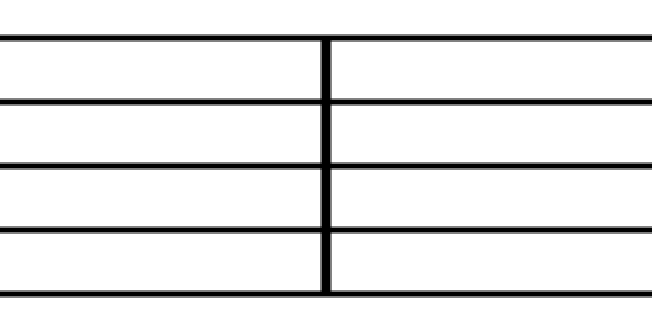
\includegraphics[width=.7\linewidth]{gfx/music-theory/barline-single.png}
      \caption{Single Bar Line}
      \label{fig:single-bar-line}
  \end{subfigure}
  \begin{subfigure}[b]{.3\linewidth}
      \centering
      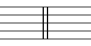
\includegraphics[width=.7\linewidth]{gfx/music-theory/barline-double.png}
      \caption{Double bar line}
      \label{fig:double-bar-line}
  \end{subfigure}
  \begin{subfigure}[b]{.3\linewidth}
      \centering
      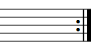
\includegraphics[width=.7\linewidth]{gfx/music-theory/barline-end-repeat.png}
      \caption{Bar line with a repeat}
      \label{fig:repeat-bar-line}
  \end{subfigure}

  \caption{An example of single, double and repeated bar lines (\cref{fig:repeat-bar-line})}
  \label{fig:bar-line-types}
\end{figure}

\subsection{Notes and Rests}

\subsubsection{Notes}
\label{sec:music-theory-notes}
Notes are used to represent duration (differentiated by their shape) and pitch (differentiated by where they're placed on the stave) of musical sounds. Most notes are comprised of a note head and a stem but may also have beams or tails in the case of notes shorter than a crotchet.

For reference, there are multiple variations in how note lengths are named and different papers refer to notes using the British and American terminology. I will be using british naming conventions throughout this project but for reference I have put both naming styles in \Cref{table:note-lengths}.

\subsubsection{Rests}
\label{sec:music-theory-rests}

Rests correspond directly to notes as you can see from \cref{table:note-lengths} but unlike notes, rests can only indicate duration and do not have pitch. They're located centred around the central (3rd) staff line and each length is represented with a different symbol or a relative location to the staff line.

\subsubsection{Duration}
\label{sec:music-theory-duration}

The note \emph{length} or \emph{value} or \emph{duration} (number of beats a note lasts for) is determined by multiple features.

A semibreve lasts 4 beats, minims 2 and crotchets 1 beat. Further divisions for quavers and semiquavers are notated by the number of tails (in the case of single, isolated notes) or the number of beams (in the case of beamed notes), both of which are located on the note stem furthest from the note head.

In general, for multiple notes with a value less than 1 the convention is to beam them together and since multiple beams can be used in place of tails you are not limited to beaming only notes of the same duration

There also exist duration dots which are single dots placed to the right of a note head or rest. These indicate that the duration of the dotted note is equal to 1.5 $\times$ the length of the original note.

\begin{table}[H]
    \renewcommand{\arraystretch}{1.8}
    \centering
    \begin{tabularx}{.7\textwidth}{ llll }
        \toprule

        Name & Name (American) & Note Symbol & Rest Symbol \\
        \midrule
        Semibreve & Whole Note      & 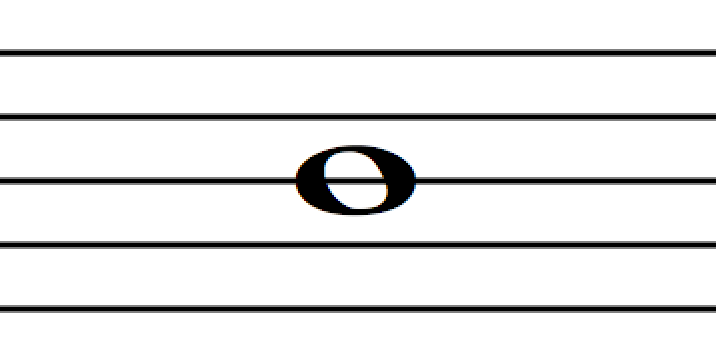
\includegraphics[height=1cm]{gfx/music-theory/notehead-semibreve.png}  & 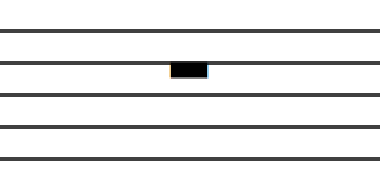
\includegraphics[height=1cm]{gfx/music-theory/rest-semibreve.png} \\
        Minim & Half Note           & 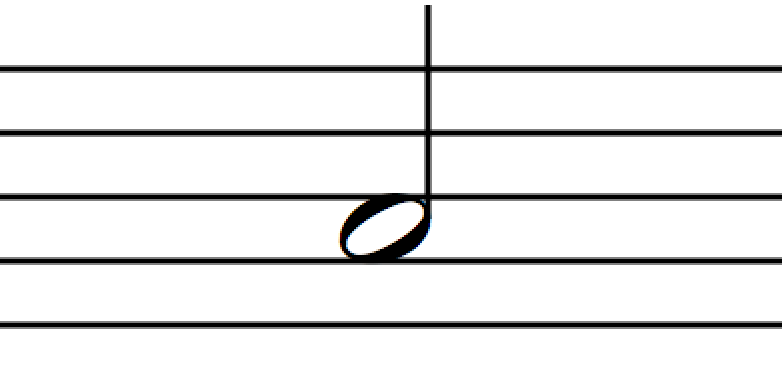
\includegraphics[height=1cm]{gfx/music-theory/notehead-minim.png}      & 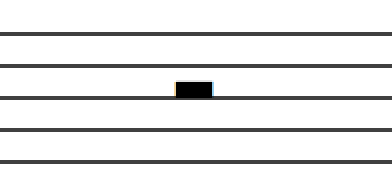
\includegraphics[height=1cm]{gfx/music-theory/rest-minim.png}     \\
        Crotchet & Quarter Note     & 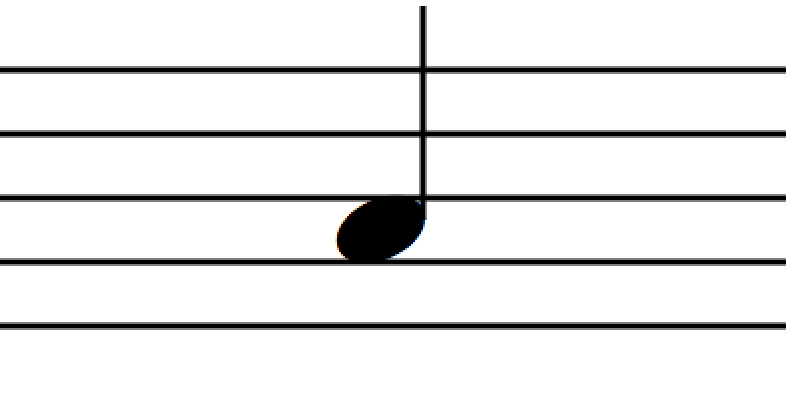
\includegraphics[height=1cm]{gfx/music-theory/notehead-crotchet.png}   & 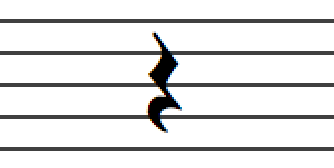
\includegraphics[height=1cm]{gfx/music-theory/rest-crotchet.png}  \\
        Quaver & Eighth Note        & 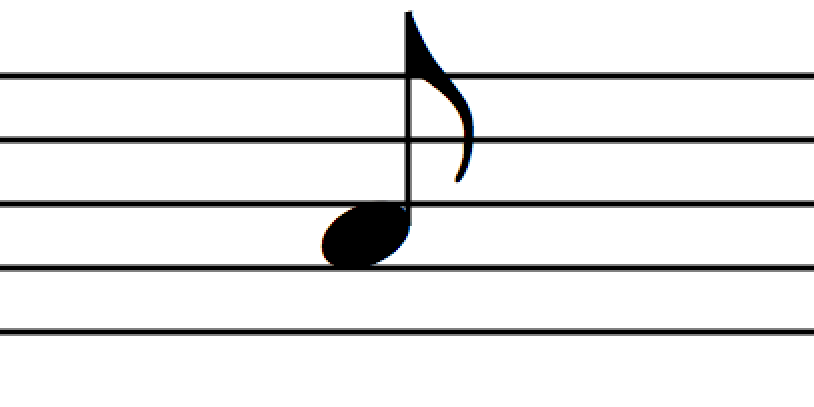
\includegraphics[height=1cm]{gfx/music-theory/notehead-quaver.png}     & 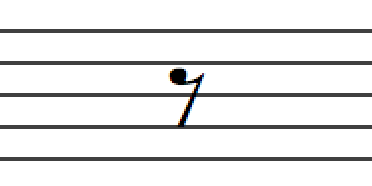
\includegraphics[height=1cm]{gfx/music-theory/rest-quaver.png}    \\
        Semiquaver & Sixteenth Note & 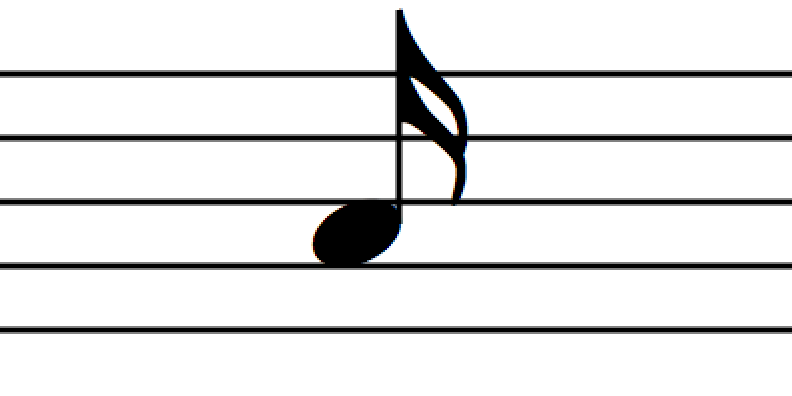
\includegraphics[height=1cm]{gfx/music-theory/notehead-semiquaver.png} & 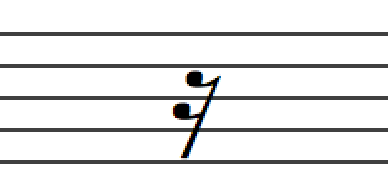
\includegraphics[height=1cm]{gfx/music-theory/rest-semiquaver.png}\\
        Duration Dot &              & 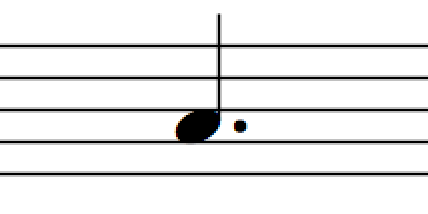
\includegraphics[height=1cm]{gfx/music-theory/notehead-dotted.png}  & 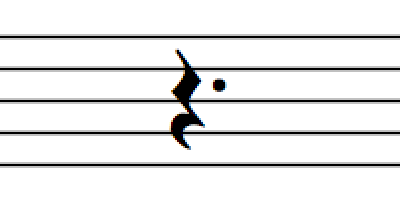
\includegraphics[height=1cm]{gfx/music-theory/rest-dotted.png} \\
        \bottomrule
    \end{tabularx}
    \caption{An overview of note and rest durations}
    \label{table:note-lengths}
\end{table}

\subsubsection{Pitch}
\label{sec:music-theory-pitch}

The absolute pitch of a note is determined by it's vertical position on the stave relative to the staff lines taking into account the clef (\cref{sec:music-theory-clefs}), the key signature (\cref{sec:music-theory-key-signatures}) and any applicable accidentals (\cref{sec:music-theory-accidentals}).

Pitch is notated by letter and number corresponding to the note itself and the octave. For example, the central C on the piano (the first ledger line on a treble clef) is noted by C4 and the next C one octave above it is notated by C5. A sequence of notes is shown labelled in \cref{fig:music-theory-pitch-labels}. For notes with sharps or naturals applied, typically an additional lowercase character (s for Sharp and b for Flat) is added, for example Fs4, Bb4 etc.

\begin{figure}[H]
  \centering
  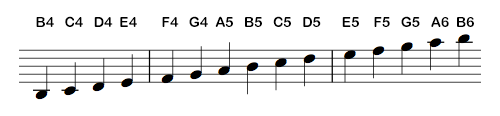
\includegraphics[width=\linewidth]{gfx/music-theory/scale.png}
  \caption{Pitch labelling for notes}
  \label{fig:music-theory-pitch-labels}
\end{figure}

\subsection{Accidentals}
\label{sec:music-theory-accidentals}
When placed on staff lines or spaces, accidentals modify the note which they precede unless cancelled out by another accidental (often a natural). There are three types of accidental: sharps, flats and naturals, which are explained in \cref{table:note-accidentals}

\begin{table}[H]
%    \def\tabularxcolumn#1{m{#1}}
    \renewcommand{\arraystretch}{1.8}
    \centering
    \begin{tabularx}{\textwidth}{ llX }
        \toprule

        Name & Symbol & Description \\
        \midrule
        Sharp   & 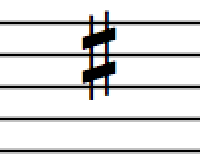
\includegraphics[width=1.5cm]{gfx/music-theory/accidental-sharp.png} & Raise the pitch of a note by one semitone\\
        Natural & 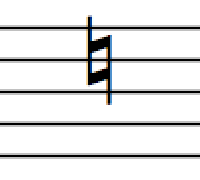
\includegraphics[width=1.5cm]{gfx/music-theory/accidental-natural.png} & Cancels any previous sharp or flat which might have applied to a note, usually from the key signature \\
        Flat    & 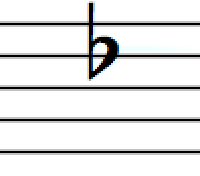
\includegraphics[width=1.5cm]{gfx/music-theory/accidental-flat.png} & Lowers the pitch of a note by one semitone \\
        \bottomrule
    \end{tabularx}
    \caption{An overview of accidentals}
    \label{table:note-accidentals}
\end{table}

\subsection{Clefs}
\label{sec:music-theory-clefs}

A clef is generally the first entity on a staff and defines the pitch range for the music, some of the most common clefs are listed below but for the scope of this project we will focus primarily on treble clef and bass clef.

\begin{table}[H]
    \renewcommand{\arraystretch}{1.8}
    \centering
    \begin{tabularx}{.4\textwidth}{ l l }
        \toprule
        Name & Symbol \\
        \midrule
        Treble Clef & 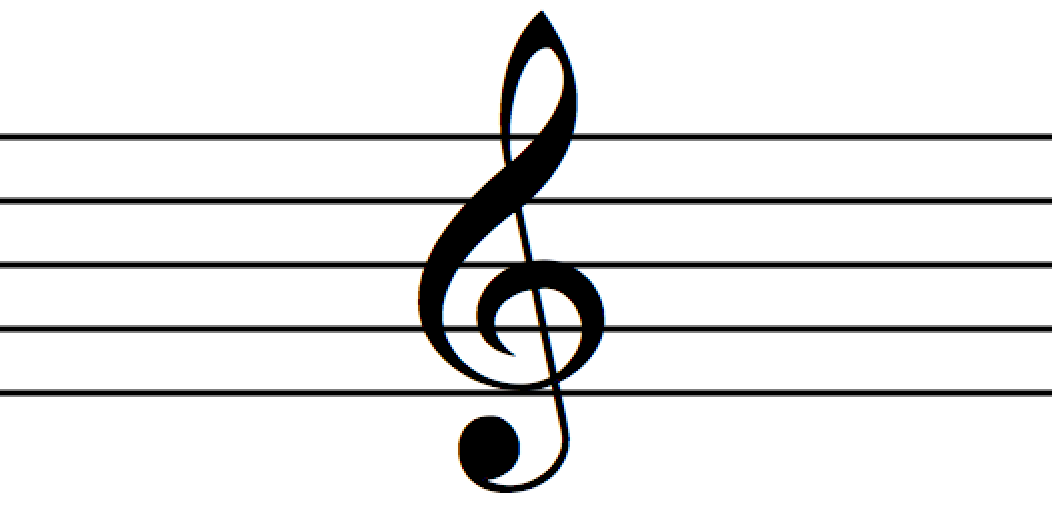
\includegraphics[height=2cm]{gfx/music-theory/clef-treble.png} \\
        Bass Clef   & 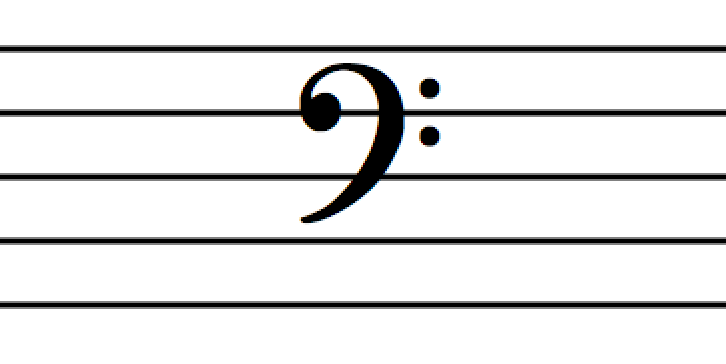
\includegraphics[height=2cm]{gfx/music-theory/clef-bass.png} \\
        \bottomrule
    \end{tabularx}
    \caption{An overview of common clefs}
    \label{table:clefs}
\end{table}

\subsection{Key Signatures}
\label{sec:music-theory-key-signatures}

Key signatures are found at the beginning of a stave next to the clef and are applicable to all musical notes which come after them, essentially setting the accidentals for the foreseeable future so we don't have to add them before every single note.

The key itself is defined by the number of sharps or flats in the signature and these follow a rigid structure and are added in a specific order left to right as shown in \cref{table:key-signatures} Sharps and flats are never combined in a key signature.

\todo[inline,color=red]{Key Signature Images}

\begin{figure}[H]
    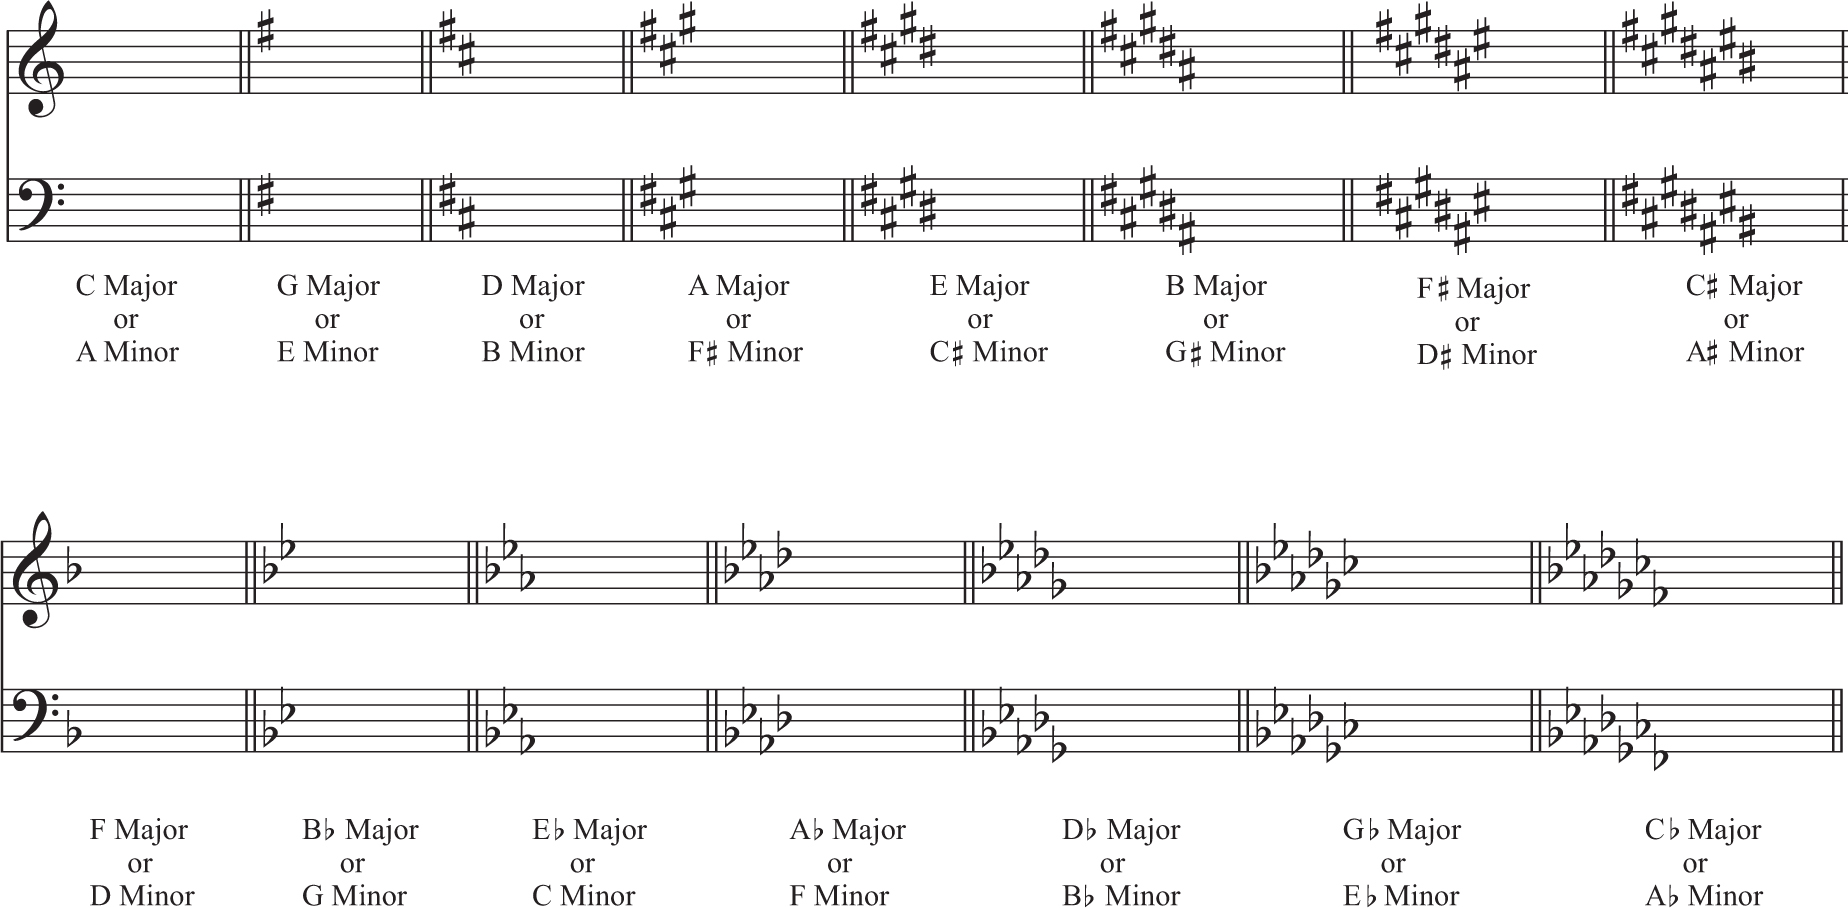
\includegraphics[width=\linewidth]{gfx/music-theory/key-signatures.jpg}
    \caption{An overview of key signatures in treble and bass clef showing the number of accidentals and the positions on the stave, from \url{http://www.netplaces.com/singing/basic-music-theory/key-signatures.htm}, accessed 10/06/2014}
    \label{table:key-signatures}
\end{figure}



\subsection{Time Signatures}
\label{sec:music-theory-time-signatures}

Time signatures can be found at the beginning of the stave or the start of a bar. The `numerator' sets the number of beats per bar and the `denominator' sets which note value is used to represent a beat for the music which follows. They can be split into several subcategories depending on the rhythm as shown in \cref{table:time-signatures}.

\begin{figure}[h!]
    \centering
    \begin{subfigure}[b]{.45\linewidth}
        \centering
        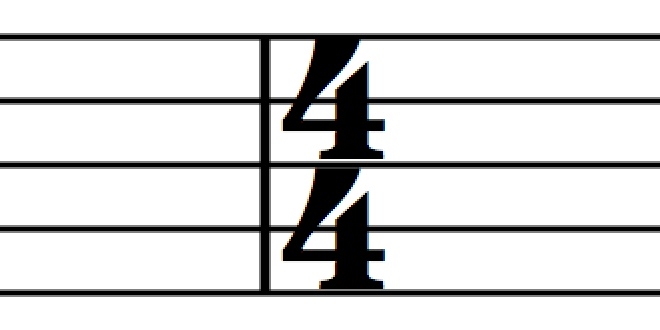
\includegraphics[height=1.8cm]{gfx/music-theory/time-signature-4-4.png}
        \caption{Four crotchets per bar}
        \label{fig:time-signature-4-4}
    \end{subfigure}
    \begin{subfigure}[b]{.45\linewidth}
        \centering
        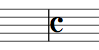
\includegraphics[height=2cm]{gfx/music-theory/time-signature-common.png}
        \caption{Common time, same as \cref{fig:time-signature-4-4}}
    \end{subfigure}
    
    \begin{subfigure}[b]{.3\linewidth}
        \centering
        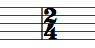
\includegraphics[height=2cm]{gfx/music-theory/time-signature-2-4.png}
        \caption{Two crotchets per bar}
    \end{subfigure}
    \begin{subfigure}[b]{.3\linewidth}
        \centering
        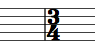
\includegraphics[height=2cm]{gfx/music-theory/time-signature-3-4.png}
        \caption{Three crotchets per bar}
    \end{subfigure}
    \begin{subfigure}[b]{.3\linewidth}
        \centering
        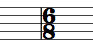
\includegraphics[height=2cm]{gfx/music-theory/time-signature-6-8.png}
        \caption{Six quavers per bar}
    \end{subfigure}

    \caption{Examples of different time signatures}
\end{figure}

